\subsection{История конструктивизма}
\begin{frame}{История конструктивизма}
    % \begin{itemize}

    % \end{itemize}


    % \begin{textblock*}{4cm}(7cm, 2cm)
    %     \begin{figure}
    %         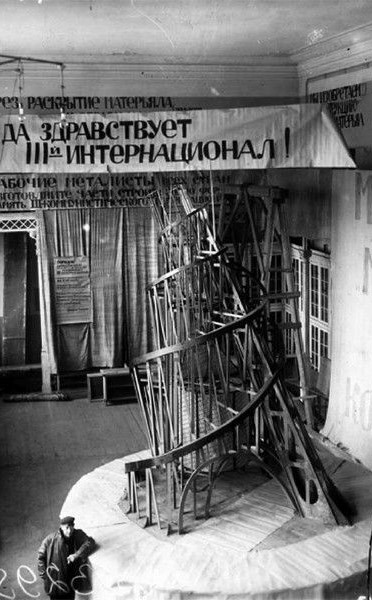
\includegraphics[height=4cm]{images/Tatlin's_Tower_maket_1919_year.jpg}
    %     \end{figure}
    % \end{textblock*}



    \begin{columns}[T,onlytextwidth]
        \begin{column}{0.56\textwidth}
            \begin{itemize}
                \item<1-> Появился на фоне значительных перемен в начале XX века
                \item<2-> Произошел в основном от супрематизма и кубофутуризма
                \item<3-> Исходная точка конструктивизма --- проект <<Памятника III Интернационала>>
                \item<4-> <<Отец конструктивизма>> --- Владимир Татлин
            \end{itemize}
        \end{column}
        \begin{column}{0.4\textwidth}
            \begin{figure}
                \centering
                \visible<3->{
                    \includegraphics<3->[width=0.7\textwidth]{images/Tatlin's_Tower_maket_1919_year.jpg}
                    \caption*{Башня Татлина}
                }
            \end{figure}
        \end{column}
    \end{columns}
\end{frame}